\documentclass[11pt,letterpaper]{article}
\usepackage[T1]{fontenc}
\usepackage[utf8]{inputenc}
\usepackage{lmodern,amsmath,amssymb,amsthm,mathtools}
\usepackage[margin=1in]{geometry}
\usepackage{microtype,booktabs,longtable,array,enumitem,xcolor,graphicx}
\usepackage{xurl,fancyhdr,needspace}
\usepackage[colorlinks=true,linkcolor=blue!45!black,citecolor=blue!45!black,urlcolor=blue!45!black]{hyperref}
\pagestyle{fancy}\fancyhf{}
\fancyhead[L]{\small Exact kernels for SubexponentialSAT}
\fancyhead[R]{\small Research review and implementation}
\fancyfoot[C]{\thepage}
\setlength{\headheight}{14pt}
\setlength{\emergencystretch}{3em}
\setlength{\parskip}{3pt}
\setlist{itemsep=3pt,topsep=5pt,leftmargin=1.5em}
\allowdisplaybreaks[2]
\newtheorem{theorem}{Theorem}[section]
\newtheorem{lemma}[theorem]{Lemma}
\newtheorem{corollary}[theorem]{Corollary}
\newtheorem{proposition}[theorem]{Proposition}
\theoremstyle{definition}\newtheorem{definition}[theorem]{Definition}
\theoremstyle{remark}\newtheorem{remark}[theorem]{Remark}
\newcommand{\OO}{\mathcal O}
\newcommand{\Aring}{\mathcal A}
\newcommand{\vv}{v_2}
\newcommand{\poly}{\operatorname{poly}}
\newcommand{\pop}{s_2}
\newcommand{\NN}{\mathbb Z_{\ge0}}
\newcommand{\coef}[2]{[\,#1\,]#2}
\newcommand{\pin}{\nolinkurl{6d3adc45061535ebe6fa7cd3d9b37dff7dcfc22a}}
\hypersetup{pdftitle={Exact kernel improvements for SubexponentialSAT},pdfauthor={Research prepared for Vladimir Reshetnikov with ChatGPT},pdfsubject={Fifteen-proposal audit, adaptive integral modes, Gray and projective coefficient extraction}}
\title{\textbf{Exact Kernel Improvements for SubexponentialSAT}\\[5pt]
\large A review of fifteen proposals, adaptive integral modes,\\
and measured improvements to packet coefficient extraction}
\author{Research prepared for Vladimir Reshetnikov\\with ChatGPT}
\date{October 26, 2026 (Pacific time)}
\begin{document}
\maketitle
\begin{abstract}
We review the recent ProveIt proposals through commit \pin, including the
eight newly placed second-round packets. One strong explicit compatible
polynomial-space construction combines asymmetric packing with full-block
Cauchy modes; the explicit normalized coefficient is approximately
$66.6051$, rather than the smallest individual displayed coefficient
$76.9090$. A compatible method using more memory has time coefficient
$44.5376$ and space coefficient $39.4959$. These are comparison baselines,
not new discoveries of this report, and neither is asserted globally optimal.

We obtain concrete improvements in two local interfaces. First, minimum-valuation
elimination on the actual real-port crossing matrix gives an integral
separation whose sorted weights dominate those of every integral rank-one
representation of that same matrix. It therefore never increases the abstract
weighted mode inventory. One checked sparse crossing block has $260$ feasible
tuples, against $3013$ for the restricted, zero-pruned, valuation-normalized
full-block Cauchy comparator. Second, we implement streamed Gray evaluation,
anisotropic centered antipodal grids, and a projective roots-of-unity
specialization for packet coefficient extraction over exact power-of-two
quotient rings. A nineteen-case suite measures $2.16$--$7.86$ times speedups
for antipodal Gray evaluation against the shipped reference routine. On a
quadratic-extension repeated-exponent case, projective evaluation reduces
$19683$ samples to $6561$ and the working precision from $41$ to $32$ bits,
with a measured $6.90$ times speedup over that reference.

The elementary identities, Gray codes, Smith forms and permanent methods
are classical. The contribution is their proved integration, precision
accounting and implementation beyond this repository snapshot. The measured
results are local-kernel timings. We do not prove a smaller unrestricted SAT
logarithmic exponent, provide a complete fast SAT solver, or certify the full
upstream ETH argument. Complete proofs of the new local interfaces, executable
checks, raw measurements and immutable source identities accompany this report.
\end{abstract}
\clearpage
\tableofcontents
\clearpage

\section{Outcome and the exact scope of the improvement}
The completed result is an exact, executable improvement to work that the
reviewed proposals perform inside their contraction engine. It has two
complementary effects: fewer abstract mode tuples for populated crossing
blocks, and less work to evaluate a packet entry for each tuple. The
underlying global counting reductions and recursive contraction identities
remain explicit dependencies.

For fixed clause width $k$, write $n$ for variables and $m$ for clauses.
The strongest justified density envelope in the reviewed corpus remains
\begin{equation}\label{eq:sat-envelope}
 \poly_k(n,m)\,
 2^{O_k\!\left(\frac{n}{\sqrt{\log n}}
       \min\{\log(2+m/n),\log\log n\}\right)}.
\end{equation}
Here and below asymptotic expressions are for sufficiently large inputs.
At fixed density $m\le Dn$ this has exponent $O_{k,D}(n/\sqrt{\log n})$; for unrestricted
density it has exponent $O_k(n\log\log n/\sqrt{\log n})$.
The $n\log\log n/\log n$ target in the precision-refinement packet depends
on an unconstructed structured-mode summation interface. It is not an
available solver whose runtime can be used as an experimentally tested
baseline \cite{index,precision,density,density2}.

Our generic coefficient algorithm improves dense grid evaluation from
$O(RqG)$ to $O(RG)$ coefficient-ring operations, after reading the input.
Here $R$ is the number of affine factors, $q$ the number of positive
homogenized target exponents and $G$ the product-grid size. Its antipodal
version evaluates only $\lfloor G/2\rfloor$ points. A supported projective
version evaluates $G/(1+\min b_j)$ points and removes factorial precision
loss. All these algorithms stream their grids and retain polynomial space.
The adaptive matrix algorithm has polynomial preprocessing cost and a
pointwise non-increase theorem for the abstract mode inventory.

These statements do not turn the measurements into full SAT runtimes.
The existing contraction proof charges packet entry work as a lower-order
term. Improving that term alone leaves its leading logarithmic order
unchanged. Dense fully populated crossing matrices also retain the known
slope-four Smith profile, so the adaptive algorithm supplies no uniform
replacement of that slope by a larger constant.

\section{Review cutoff, proposal inventory and combined baseline}
\label{sec:review}
The review began at ProveIt commit
\nolinkurl{ab2fbc9e03d5c3d0ad6dec8686960bfe498b0b06}.
At that point there were seven indexed packets and seven incoming archives.
A closing check found one further matching-packing packet, followed by the
placement commit \pin. We read that additional report and relevant code.
The final inventory is fifteen packets. At the closing snapshot
\texttt{docs/incoming/} contains its index and the research packets are
under \texttt{Computability/SubexponentialSAT/Research/}.

The vendored preprint is pinned upstream to
\nolinkurl{7ef5c0cc5ca4b0e072b7a050fca09ab24bc6fa3a}.
The repository's own trust statement says that placement did not verify
the mathematical results or run a formal development. This report performs
a scoped analytic and interface review; it does not replace that statement
with a claim of full formal verification \cite{index,placement,preprint}.

\subsection{What each packet contributes}
In the next table, coefficients refer to the normalized contraction scale
\begin{equation}\label{eq:normalization}
 \poly(s+\mathcal L)\,2^{(C+o(1))s/\sqrt{\log_2s}},
\end{equation}
where $s$ bounds root Boolean wires, initial precision and truncation order,
the root degree is at most $\lceil s^{9/10}\rceil$, and $\mathcal L$ is the
description length. They are not numerical coefficients on SAT variables.

\small
\begin{longtable}{@{}p{.25\textwidth}p{.45\textwidth}p{.22\textwidth}@{}}
\toprule Packet & Contribution retained in the comparison & Limit\\\midrule
\endfirsthead
\toprule Packet & Contribution retained in the comparison & Limit\\\midrule\endhead
Contraction improvements & Exact taper, leading precision $6MD/u$, coefficient
$648.4411$, streamed homogeneous finite differences. & No measured solver.\\[4pt]
Factorial Cauchy modes & Integral modes with slope three. & Same logarithmic order.\\[4pt]
Precision refinement & Exact recovery losses and real taper minimax. & Faster summation is conditional.\\[4pt]
SAT density improvement & Uniform density envelope \eqref{eq:sat-envelope}. & No better unrestricted order.\\[4pt]
ETH density refinement & Related density bound and local odd-unit Smith profile. & Local profile alone is not all-level grouping.\\[4pt]
Scalar parity refinement & Scalar lift and smaller incidence-degree cap. & New factorization still missing.\\[4pt]
Asymptotic analysis & Restricted barriers and explicit missing interfaces. & No improved unrestricted algorithm.\\[4pt]
Recursive refinement & $133.2074$; missing-residue Cauchy slope $64/21$. & Some finite inventories worsen.\\[4pt]
Packet refinement & $95.6639$; nearly balanced loads and additive precision guard. & Same order.\\[4pt]
High moments & $94.7482$ via moment control; degree-sensitive specializations. & Setup cost and eventual thresholds matter.\\[4pt]
Balanced packing & $94.7482$ via constructive two-stage balancing. & Same order.\\[4pt]
Matching refinement & $94.7482$ via matching potentials and thin gaps. & Additional late packet; no new extraction routine.\\[4pt]
Round-two refinement & $84.0663$; exact crossing fraction and two-stage alphabet. & No completed stronger-order interface.\\[4pt]
Asymmetric balancing & $76.9090$; uses smaller fresh-side degree below the root. & Its displayed basis has slope three.\\[4pt]
Joint Cauchy & All-level full crossing-block slope four. Individual coefficient
$319.6858$; cached/Strassen option $225.5971$. & Its own schedule is weaker; cached option uses more memory.\\
\bottomrule
\end{longtable}
\normalsize

The separate $49$-page manuscript credited to Claude has the same relevant
unrestricted logarithmic order and does not provide a directly comparable
explicit coefficient on \eqref{eq:normalization}. Numerical domination of
that independent algorithm is therefore not established here. The inherited
OpenAI manuscript's Appendix D is the comparison target, rather than the
weaker endpoint described by its archived Lean scope material.

\subsection{Combine compatible ingredients before claiming a gain}
Asymmetric packing supplies near-unit padding, at most
\[
 (2(1-1/r)+o(1))M/D
\]
families, child size $(2/r+o(1))M$, and precision $(6+o(1))MD/u$.
The joint Cauchy basis has the same source and target groups, the same
family multiplicity, and weights
\[
 a+1-i+4j-2\pop(j).
\]
It changes neither child wiring nor the fresh-side degree. Substituting
it for the slope-three basis multiplies the leading entropy coefficient
by $\sqrt3/2$ \cite{asym,joint}.

For the explicit asymmetric schedule $r=16$,
\[
 u_0=\lfloor\lambda/81\rfloor,\qquad
 u_d=\left\lfloor\frac{\lambda}{108\,4^{d-1}}\right\rfloor\quad(d\ge1),
 \qquad\lambda=\lceil\log_2s\rceil,
\]
the resulting coefficient is
\begin{equation}\label{eq:composed-ps}
 C_{\rm poly}=\frac{\pi\sqrt{15/8}}{\ln2}(9+\sqrt3)
 =66.6051434076\ldots .
\end{equation}
The boundary version of its fixed-$r=16$ family approaches
$66.1927236936$. A further numerical optimization of a two-stage family
gives approximately $66.12047546$ with root alphabet $17$ and tail alphabet
$13$. This last number is recorded as a schedule-model infimum, not as a
new implementation theorem. None of these values is a lower bound or a
global optimum over all schedules. Our practical comparison does not rely
on advertising a modest schedule retuning as a structural breakthrough.

When more memory is allowed, the joint packet's exact-weight indexing,
cached group contractions, and three-block Strassen construction also
compose with this schedule. For $r=16$ split the groups into $5,5,6$.
Set
\[
 K_0=\frac{9\pi\sqrt2}{\ln2},\quad
 A=\sqrt{30/256},\quad B=\sqrt{150/256},\quad J=\sqrt{120/256},
\]
and, with $\omega=\log_2 7$,
\[
 S=\sqrt{\frac{170-[1-(\omega-2)^2]50}{256}}.
\]
The directed inter-block pair counts are $50,60,60$.
The first child scale is $K_1/K_0=\sqrt3/12$; subsequent scales have ratio
$1/4$. In the recurrence, cached child evaluations contribute
$A K_d$ before the recursive cost, and table/matrix work contributes
$\max(B,S)K_d$. Since
$A+S\sqrt3/12<S$ and $A(1+\sqrt3/9)<S$, the root matrix work dominates.
Thus one available combined comparison has
\begin{equation}\label{eq:composed-exp}
 C_{\rm time}=K_0S=44.5375718550\ldots,\qquad
 C_{\rm space}=K_0J=39.4959495337\ldots .
\end{equation}
This is a different space regime from \eqref{eq:composed-ps}. The numerical
calculation and its assumptions are reproducible in the accompanying code.

\section{Exact packet coefficient extraction}
\label{sec:extraction}
Let $f\in\mathbb Z[U]$ be monic and $\ell\ge1$. Work over
\[
 \Aring_p=(\mathbb Z/2^p\mathbb Z)[U,V]/(f(U),V^\ell).
\]
For this section $f$ may be reducible and the ring may contain nilpotents.
Its integral version is free as a $\mathbb Z$-module in the usual monomial
basis, so coordinatewise exact division after sufficient precision is valid.

Given $R$ affine forms, the required entry is
\begin{equation}\label{eq:target}
 c_\beta=[Z^\beta]\prod_{r=1}^R
 \left(a_{r0}+\sum_{j=1}^q a_{rj}Z_j\right)\pmod{2^p}.
\end{equation}
An impossible target $|\beta|>R$ gives zero. Otherwise put
\[
 b=(R-|\beta|,\beta_1,\ldots,\beta_q),\qquad
 H(X)=\prod_{r=1}^R\sum_j a_{rj}X_j,
\]
so that $|b|=R$ and $c_\beta=[X^b]H$. A coordinate with $b_j=0$ can be
set to zero and removed from all evaluation loops. Below, $q$ denotes the
number of remaining positive coordinates. Define
\begin{equation}\label{eq:grid-parameters}
 G=\prod_j(b_j+1),\qquad
 \nu=\sum_j\vv(b_j!)=\sum_j(b_j-\pop(b_j)),\qquad
 O=\sum_{j:\,b_j\text{ odd}}b_j.
\end{equation}
The shipped finite-difference implementation uses exactly $G$ grid points
and working precision $p+\nu$ \cite{extraction}. It recomputes each of the
$R$ row values from every grid coordinate at every point. The inspected
later proposals retain this routine or the older direct row expansion;
none supplies the three implementations introduced here.

\subsection{Gray traversal without any precision change}
A reflected mixed-radix Gray traversal changes exactly one coordinate by
$+1$ or $-1$ at each transition. If $L_r=\sum_j a_{rj}\gamma_j$ is the
current row value, changing coordinate $j$ by $\varepsilon$ updates it by
\[
 L_r\longleftarrow L_r+\varepsilon a_{rj}.
\]
Only $R$ row updates are needed. The signed binomial weight can also be
updated without recomputing its product. For an increasing coordinate,
\[
 w_{\rm new}=w_{\rm old}\frac{b_j-\gamma_j}{\gamma_j+1},
\]
and the decreasing formula is analogous. The division is an exact integer
division of the entire positive weight, followed by a sign flip. It is not
division by a possibly even residue in $\Aring_p$.

\begin{proposition}[Streaming arithmetic cost]\label{prop:gray}
For $R>0$, full-grid Gray evaluation computes \eqref{eq:target} at the same
$p+\nu$ working precision as the shipped reference, with $G$ evaluations
and $O(\text{input size}+RG)$ coefficient-ring operations. It stores the
input, one grid point, $R$ row values, one integer weight and one accumulator.
\end{proposition}
\begin{proof}
Initialize all row values at the initial grid point. Each of the $G-1$
transitions uses $R$ additions/scalings. At each point the product uses
$R$ ring multiplications, followed by one weighted accumulation. The
standard finite-difference identity is unchanged. The integer weight has
at most $R+1$ bits, because the product of binomial coefficients is at
most $2^R$. The mixed-radix counter can scan $O(q)$ positions on one
transition, but its aggregate work over a grid with all radices at least
two is $O(G)$, by the geometric bound on carries. No worst-case constant
delay assertion is needed.
\end{proof}

\subsection{Anisotropic centered grids and exact antipodal pairing}
Choose the smallest positive integer step that centers the grid integrally:
\begin{equation}\label{eq:steps}
 h_j=\begin{cases}1,&b_j\text{ even},\\2,&b_j\text{ odd},\end{cases}
 \qquad x_j(\gamma_j)=h_j\gamma_j-h_jb_j/2.
\end{equation}
Define $w(\gamma)=(-1)^{R-|\gamma|}\prod_j\binom{b_j}{\gamma_j}$.

\begin{theorem}[Anisotropic antipodal extraction]\label{thm:antipodal}
Assume $R>0$. Let $\mathcal P$ contain one representative of each
noncentral pair $\{\gamma,b-\gamma\}$ in the product grid. Then
\begin{equation}\label{eq:antipodal-identity}
 \sum_{\gamma\in\mathcal P}w(\gamma)H(x(\gamma))
 =\left(2^{O-1}\prod_j b_j!\right)[X^b]H.
\end{equation}
The parenthesized integer has valuation $\nu+O-1\ge0$. Consequently
the target coefficient modulo $2^p$ can be recovered from exactly
$\lfloor G/2\rfloor$ evaluations at working precision
\begin{equation}\label{eq:antipodal-precision}
 P=p+\nu+O-1.
\end{equation}
\end{theorem}
\begin{proof}
The product of the $b_j$-th finite-difference operators annihilates every
monomial having exponent below $b_j$ in at least one coordinate. Since
$H$ is homogeneous of total degree $|b|$, the only surviving monomial is
$X^b$. Its product difference equals $\prod_j b_j!h_j^{b_j}$.
Thus the full-grid sum equals $2^O\prod_j b_j![X^b]H$.

Complementation sends $x$ to $-x$. It changes the signed binomial weight
by $(-1)^R$ and the value of $H$ by the same factor. The two contributions
therefore agree. An unpaired center exists only when all $b_j$ are even;
there $x=0$ and $H(0)=0$ for $R>0$. Pairing proves
\eqref{eq:antipodal-identity} as an identity over the integers.
If $O>0$ then $O\ge1$. If $O=0$, at least one positive exponent is even,
so $\nu\ge1$. The denominator is consequently integral in both cases.

Fix the original coefficient representatives at creation precision $p$.
Compute the representative sum modulo $2^P$. Its coordinates are divisible
by $2^{\nu+O-1}$. Divide those canonical integer coordinates by this
power of two and multiply by the inverse of the odd part of
$\prod_j b_j!$ modulo $2^p$. Errors before division are multiples of
$2^P$, hence errors after division are multiples of $2^p$. Freeness of
the integral quotient algebra justifies the coordinatewise operation.
No even element is inverted.
\end{proof}

Three cases make the precision effect transparent:
\begin{center}
\begin{tabular}{@{}lll@{}}
\toprule Target pattern & Evaluations & Working precision\\\midrule
All positive $b_j$ even & $(G-1)/2$ & $p+\nu-1$\\
Exactly one odd exponent, equal to $1$ & $G/2$ & $p+\nu$\\
All positive $b_j=1$ & $2^{R-1}$ & $p+R-1$\\\bottomrule
\end{tabular}
\end{center}
The last line is the classical Glynn permanent specialization. The squarefree
case pays more precision even though it uses half as many points. The
all-even case uses one fewer bit than the old full grid.

\begin{proposition}[Optimal integer centered step valuation]
Among symmetric arithmetic grids with integer coordinates and lengths
$b_j+1$, the choice \eqref{eq:steps} minimizes the two-adic valuation
of the difference denominator. The loss $\nu+O-1$ is sharp for this
paired functional.
\end{proposition}
\begin{proof}
An integer-centered grid requires $h_jb_j$ even. An odd $b_j$ forces
$\vv(h_j)\ge1$; an even $b_j$ allows $h_j=1$. This gives the minimum
$\sum_jb_j\vv(h_j)=O$. For $H=X^b$ the coefficient is one and the
representative numerator equals the displayed denominator, proving the
sharpness statement for this functional.
\end{proof}

\subsection{Streaming the half-grid}
If an exponent $b_j$ is odd, restrict that coordinate to
$0\le\gamma_j\le(b_j-1)/2$ and leave all others unrestricted. This is
one rectangular set containing exactly one point of each pair. If all
exponents are even, use a disjoint union of boxes: earlier coordinates
are fixed at their midpoints, the first noncentral coordinate $j$ lies
strictly below its midpoint, and subsequent coordinates are unrestricted.
This covers $(G-1)/2$ representatives and omits only the zero center.

Each box admits reflected Gray traversal. Row values need initialization
at most $q$ times. The total initialization cost is $O(Rq^2)$, absorbed
by $O(RG)$ because an all-even positive profile has $G\ge3^q$.
Within a box each transition updates row $r$ by
$\pm h_j a_{rj}$. The storage remains polynomial. Degree zero and
impossible targets are handled directly, outside the paired formula.

\section{Projective roots-of-unity extraction}
\label{sec:projective}
The half-grid is not always the smallest useful grid. Homogeneity can
remove a whole coordinate, provided the other coordinate filters have
the required orthogonality. This is related to classical generalized
permanent identities and monomial Waring decompositions
\cite{glynn,chin,ccg}. We give the exact modular form needed here.

\begin{theorem}[Projective coefficient filter]\label{thm:projective}
Let $H$ be homogeneous of degree $R=\sum_jb_j$, with all retained
$b_j>0$. Choose $k$ with $b_k=\min_j b_j$. Put $d_j=b_j+1$.
For every $j\ne k$, suppose a ring element $\omega_j$ satisfies
\begin{equation}\label{eq:orthogonality}
 \omega_j^{d_j}=1,\qquad
 \sum_{t=0}^{d_j-1}\omega_j^{tm}
 =\begin{cases}d_j,&d_j\mid m,\\0,&d_j\nmid m.\end{cases}
\end{equation}
The identities may hold exactly or modulo a chosen working power of two.
With $X_k=1$ and $X_j=\omega_j^{t_j}$ for $j\ne k$,
\begin{equation}\label{eq:projective-identity}
 \sum_{\substack{0\le t_j<d_j\\j\ne k}}
 \left(\prod_{j\ne k}\omega_j^{-b_jt_j}\right)H(X)
 =\left(\prod_{j\ne k}d_j\right)[X^b]H.
\end{equation}
There are exactly $G/(1+\min b_j)$ evaluations. To recover modulo
$2^p$, sufficient working precision is
\begin{equation}\label{eq:projective-precision}
 P=p+\sum_{j\ne k}\vv(d_j).
\end{equation}
\end{theorem}
\begin{proof}
Expand $H$. Orthogonality retains a monomial $X^\alpha$ only when
$\alpha_j\equiv b_j\pmod{d_j}$ for $j\ne k$. Since $0\le b_j<d_j$
and $\alpha_j\ge0$, this means $\alpha_j=b_j+t'_jd_j$ with $t'_j\ge0$.
Homogeneity gives $\alpha_k=b_k-\sum_{j\ne k}t'_jd_j$.
Every $d_j=b_j+1$ exceeds $b_k$. Thus any positive $t'_j$ would force
$\alpha_k<0$, and the only surviving monomial is $X^b$.
Its contribution is $\prod_{j\ne k}d_j$ times its coefficient.
If the identities hold only modulo $2^P$, the same proof is a congruence
modulo $2^P$. Divide canonical integer coordinates by the explicit power
of two in the denominator and invert its odd part. The precision loss
is exactly the sum in \eqref{eq:projective-precision}.
\end{proof}

Choosing a minimum exponent is essential. For example, fixing the exponent-two
coordinate in target $X_0^2X_1$ and sampling $X_1$ only at $\pm1$ aliases the
monomial $X_1^3$. Mere multiplicative order is also insufficient over an
arbitrary ring; the required assertion is the orthogonality in
\eqref{eq:orthogonality}.

\subsection{Implemented specialization: exponents one and two}
For $b_j=1$ use roots $1,-1$. For $b_j=2$ use $1,\omega,\omega^2$ with
$\omega^2+\omega+1=0$. These imply the needed orthogonality in every
commutative ring. The code verifies the cubic relation at the working
precision. For the existing ring defined by $f(U)=U^2+U+1$, the element
$\omega=U$ supplies the root directly, including with a truncated $V$ axis.
No extra extension dimension is allocated implicitly.

If there are $q_1$ exponents equal to one and $q_2$ equal to two, then:
\begin{center}
\begin{tabular}{@{}lll@{}}
\toprule Pattern & Evaluations & Working precision\\\midrule
$q_1>0$ & $2^{q_1-1}3^{q_2}$ & $p+q_1-1$\\
$q_1=0$ & $3^{q_2-1}$ & $p$\\\bottomrule
\end{tabular}
\end{center}
In the mixed case the evaluation count matches the paired grid, while
the precision saves $q_2$ bits. In the all-two case it saves almost another
factor $3/2$ in samples and removes all factorial precision loss.

The source contraction uses an unramified residue extension of degree
$e=4\lceil\log_2s\rceil$. Since $e$ is even, its residue field contains
the nontrivial cubic roots. A chosen residue root lifts modulo $2^P$ because
the derivative $2\omega+1$ is a unit. This is a finite-precision Hensel
statement; it does not assert that the uncompleted rational coefficient
field already contains an exact complex cube root. A caller using a
different defining polynomial supplies a correctly lifted root. The
provided general theorem also describes other supported odd root orders;
the executable specialization deliberately restricts positive exponents
to one and two.

Reflected Gray traversal of the root-index grid again changes one coordinate.
Precompute each adjacent root difference times each row coefficient.
Then one transition uses $R$ additions; the character weight updates by a
unit root multiplication. The loop has $O(RG/(1+\min b_j))$ ring
operations, plus polynomial initialization, and polynomial storage.

\section{Adaptive integral modes on actual crossing blocks}
\label{sec:adaptive}
The other improvement changes which modes exist before any packet-entry
coefficient is requested. The full-block basis uses a convenient ordering
of padded slots. Restricting it to real ports leaves cancellations and
linear dependencies that pointwise source/target valuation normalization
does not remove.

For this section the kernel coefficients belong to the unramified chain
ring
\[
 R_p=(\mathbb Z/2^p\mathbb Z)[U]/(f(U)),
\]
where $f\bmod2$ is irreducible. The two-adic valuation of a nonzero element
is the minimum coordinate valuation; zero has capped valuation $p$.
An element of valuation zero is a unit. The kernel matrix itself contains
no nilpotent $V$ dependence. The surrounding tensor entries may still
belong to $R_p[V]/(V^\ell)$.

\subsection{Minimum-valuation elimination}
Let $K$ be the $m\times n$ matrix of one actual crossing orientation,
restricted to its real row and column slots. At a residual matrix $E$,
choose an entry $E_{ij}$ of minimum valuation $e<p$. Write
$E_{ij}=2^e u$ with $u$ a unit at precision $p-e$. Define
\[
 c_h=E_{hj},\qquad
 r_k=(E_{ik}/2^e)u^{-1}\pmod{2^{p-e}}.
\]
Use canonical lifts of the $r_k$ to $R_p$ and subtract $cr^{\mathsf T}$.
The pivot row and column vanish modulo $2^p$. Repeating gives
\begin{equation}\label{eq:adaptive-separation}
 K=\sum_{h=1}^{t}c_h r_h^{\mathsf T}\pmod{2^p},\qquad
 \vv(c_h)\ge e_h,
 \quad e_1\le\cdots\le e_t<p.
\end{equation}
The extra precision needed to prepare a Cauchy kernel is a separate matter;
the elimination itself never requests more than the matrix's $p$ bits.

\begin{theorem}[Exact adaptive separation and its cost]\label{thm:smith}
The algorithm above produces the nonzero Smith valuations of $K$ and an
integral rank-one separation with those weights. It takes
$O(mn\min(m,n))$ ring operations, in addition to polynomial-time unit
inversions, and $O(mn)$ stored ring elements.
\end{theorem}
\begin{proof}
Every residual entry is divisible by $2^e$. The quotient pivot is a unit,
so the displayed row is integral at precision $p-e$. Since the entire pivot
column is divisible by $2^e$, ambiguity in lifting that row changes its
outer product only by a multiple of $2^p$. Direct substitution proves
that the pivot row and column become zero.

Equivalently, swap the pivot to the top-left position, subtract integral
multiples of its row and column and normalize the odd unit. These are
invertible row and column operations over the chain ring. The result is a
diagonal entry $2^e$ and a smaller residual matrix. Every residual entry
remains divisible by $2^e$, so subsequent pivot valuations cannot decrease.
Induction therefore gives the Smith diagonal and the exact decomposition.
There are at most $\min(m,n)$ pivots, each requiring a scan and a rank-one
update of $O(mn)$ entries. The sum of stored source and target vector
lengths is at most $\min(m,n)(m+n)=O(mn)$, in addition to the matrix.
\end{proof}

\subsection{A pointwise comparison against every integral separated basis}
\begin{theorem}[Weight-profile domination]\label{thm:domination}
Suppose another integral representation of this same matrix is
\[
 K=\sum_{j=1}^{N}2^{w_j}a_jb_j^{\mathsf T}\pmod{2^p},
 \qquad 0\le w_1\le\cdots\le w_N<p.
\]
Let $e_1\le\cdots\le e_t$ be the adaptive weights. For every
$1\le q\le p$,
\begin{equation}\label{eq:cumulative-domination}
 \#\{h:e_h<q\}\le\#\{j:w_j<q\}.
\end{equation}
In particular $t\le N$ and $e_h\ge w_h$ for $1\le h\le t$.
If all weights are positive, then for any budget $1\le P\le p$,
\begin{equation}\label{eq:inventory-domination}
 \#\{\beta\in\NN^t:\sum_he_h\beta_h<P\}
 \le
 \#\{\beta\in\NN^N:\sum_jw_j\beta_j<P\}.
\end{equation}
\end{theorem}
\begin{proof}
Reduce the matrix modulo $2^q$. Its Smith image is a direct sum of exactly
$t_q=\#\{h:e_h<q\}$ nonzero cyclic chain-ring modules. Thus its minimal
number of generators is $t_q$. In the alternative representation all
terms with $w_j\ge q$ vanish. The image is contained in the submodule
generated by the $N_q=\#\{j:w_j<q\}$ surviving target columns.

For completeness, submodule containment does bound the number of
generators here. A finite module over a chain ring is a direct sum of
cyclic modules. Its minimum generator number equals the dimension over
the residue field of its socle, the submodule annihilated by $2$.
Inclusion of modules gives inclusion of their socles. Hence a submodule
of a module generated by $N_q$ elements needs at most $N_q$ generators.
This proves \eqref{eq:cumulative-domination}. Taking $q=p$ proves
$t\le N$; if $e_h<w_h$, taking $q=e_h+1$ contradicts the cumulative
inequality. Finally map a feasible adaptive exponent tuple to its first
$t$ coordinates in the alternative system and append zeros. The total
alternative weight is no larger, proving the injection in
\eqref{eq:inventory-domination}.
\end{proof}

This is a theorem about separated representations of a fixed matrix.
It does not claim optimality of every way of contracting a tensor network,
or of nonlinear cancellation among full mode tuples. It is stronger than
a comparison only with untrimmed padded modes: it still applies after
restricting an earlier basis to real ports, deleting zero terms and
transferring every common source valuation into the target coefficient.

The matrix row and column sets lie within one source/target orientation.
Every new source form therefore depends on the same source group's bits,
and every new target coefficient belongs to the same target group.
Freeze the generated source and target vectors as canonical representatives
at their creation precision; later recursive precision increases reuse
these same representatives. The exact factorization used in the source
recursion survives. The degree,
wire and packing invariants also survive. Polynomial setup cost and
polynomial matrix storage are admissible because packet length is a
fixed power of the root size in the supplied schedules.

\subsection{A closed-form family with strictly stronger slopes}
The preceding algorithm has a transparent special case. Fix a valuation
level $i$, and let real row and column slots be
$x_0+Hj$, $0\le j<N$, with $\vv(H)=i+h$, $h\ge1$.
Write $T=2^i\tau$ with $\tau$ a unit and $H=2^{i+h}v$ with $v$ odd.
The crossing matrix is
\[
 K_{jk}=\frac{\Gamma(T)/2^i}{\tau+2^hv(j-k)},
 \qquad \Gamma(T)=\mathcal C(T)/\mathcal C'(0).
\]
Let $\delta=\vv(\Gamma(T)/2^i)$; for unit $\zeta$, including the
extension-field values used in the examples, $\delta=a+1-i$.

\begin{corollary}[Dyadically spaced real ports]\label{cor:stride}
The nonzero Smith weights, truncated at precision $p$, are
\begin{equation}\label{eq:stride}
 e_j=\delta+2hj+2\vv(j!)
     =\delta+(2h+2)j-2\pop(j),\qquad 0\le j<N.
\end{equation}
\end{corollary}
\begin{proof}
Apply Cauchy elimination in the actual consecutive real-slot order.
All denominators are units after division by $2^i$.
The target factor after $j$ pivots contains
$\prod_{k<j}2^hv(j-k)$, of valuation $hj+\vv(j!)$,
and so does the source factor. For a later row index $l\ge j$,
$\prod_{k<j}(l-k)=j!\binom{l}{j}$ is divisible by $j!$, with equality
of valuations at $l=j$; entries before the diagonal vanish. The same
argument applies on the column side. Dividing these known powers leaves
triangular transformations with unit diagonals. The pivot therefore
has valuation \eqref{eq:stride}; the normalized triangular matrices
are invertible. Equivalently, the Cauchy determinant formula and
Vandermonde products show that consecutive principal minors attain
the minimum determinant valuations at every order.
\end{proof}
The full padded profile corresponds to $h=1$ and slope four. Slots
spaced an additional factor $2^{h-1}$ have slope $2h+2$ on this block.
That is a real structural gain for the stated support pattern. General
SAT encodings are not proved to generate this pattern uniformly, so it
does not change \eqref{eq:sat-envelope}.

\section{Executed evidence: correctness and measured performance}
\label{sec:evidence}
The benchmark programs use Python 3.12.14 on the provided Linux x86-64
execution environment. They use only the standard library, fixed seeds,
three timed repetitions, and rotated method order. Each timing fixture is
checked against direct truncated polynomial multiplication outside the
timed region. The full coefficients, seeds, ring specifications,
precisions, raw repetitions and medians are included in the JSON data.
The cases are deterministically generated packet-kernel inputs, not a
sample of SAT formulas or a representative industrial benchmark suite.

\subsection{Coefficient extraction measurements}
\begin{table}[htbp]
\centering\small
\begin{tabular}{@{}lrrrrr@{}}
\toprule
Case & $R$ & Old & Gray & Antipodal & Gain\\\midrule
Squarefree & 14 & 1.815878 & 0.509625 & 0.231138 & 7.86\\
All exponents two & 18 & 2.371582 & 0.759171 & 0.407105 & 5.83\\
Three exponents sixteen & 48 & 0.970922 & 0.462456 & 0.278199 & 3.49\\
One odd exponent & 13 & 0.095707 & 0.038842 & 0.019302 & 4.96\\
Quadratic extension & 10 & 0.071759 & 0.034595 & 0.014858 & 4.83\\
Nilpotent extension & 8 & 0.021168 & 0.012678 & 0.006339 & 3.34\\
\bottomrule
\end{tabular}
\caption{Selected packet extraction medians in seconds. Gain is the old runtime divided by the antipodal runtime; it is not a SAT speedup.}
\end{table}

Across the nineteen cases in the general extraction suite, the median
of the per-case speedup ratios for antipodal Gray evaluation is
$4.56$, with observed range $2.16$--$7.86$. The column labelled ``Gray''
retains the old working precision and shows the benefit of incremental
row evaluation separately from symmetry.

\begin{figure}[htbp]
\centering
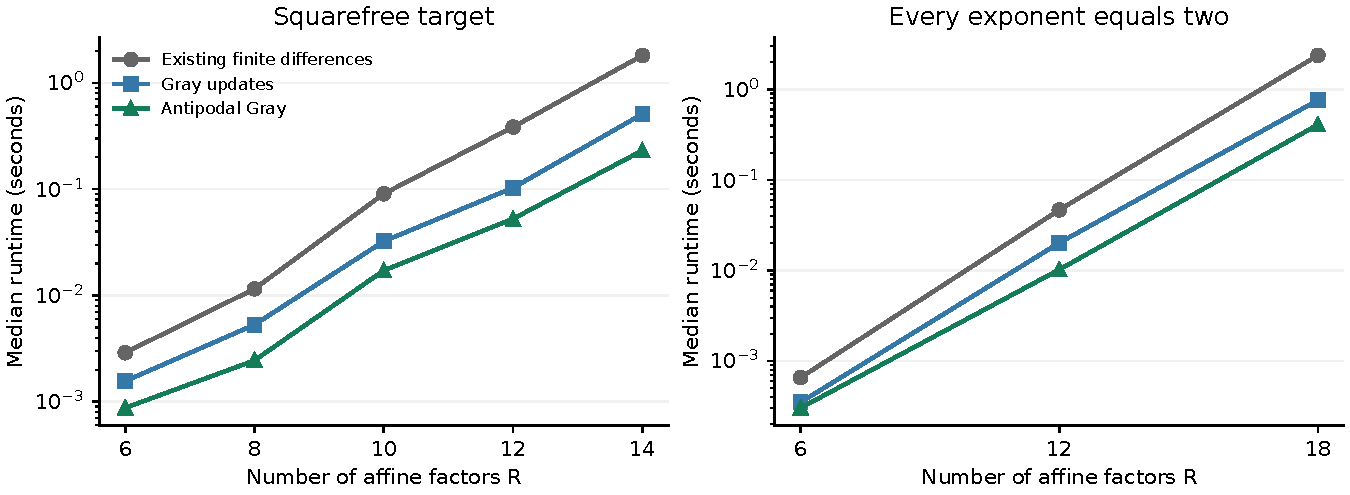
\includegraphics[width=.98\textwidth]{figures/extraction_scaling.pdf}
\caption{Measured scalar packet-entry runtimes, medians of three runs.
Both panels are logarithmic in time. These are local coefficient extractions,
not SAT solve times. The paired-exponent method also uses one fewer working
bit than the old full grid.}
\label{fig:scaling}
\end{figure}

\begin{table}[htbp]
\centering\small
\begin{tabular}{@{}lrrrrr@{}}
\toprule
Case & $R$ & Old & Antipodal & Projective & Gain\\\midrule
All two, small & 6 & 0.000980 & 0.000333 & 0.000345 & 2.84\\
All two, quadratic & 18 & 2.914805 & 0.553943 & 0.422439 & 6.90\\
All two, nilpotent & 12 & 0.080007 & 0.024649 & 0.017121 & 4.67\\
All two, $p=1$ & 12 & 0.044650 & 0.009691 & 0.006115 & 7.30\\
Mixed one/two & 10 & 0.018711 & 0.005157 & 0.005131 & 3.65\\
\bottomrule
\end{tabular}
\caption{Projective specialization, median seconds. The same extension ring and same coefficient input are used for all methods within each row. Gain compares old and projective runtimes.}
\end{table}

The projective suite contains ten cases. Its all-two profiles improve on
the antipodal kernel by approximately $1.31$--$1.58$ times in the larger
tested cases. Mixed one/two profiles have the same sample count and are
approximately tied; the tiny three-axis all-two case is slightly slower
than antipodal evaluation. The data therefore support a dispatchable
specialization, not a claim that it is universally fastest. All comparisons
use the same coefficient ring in each row. We do not compare a scalar-ring
method against a method silently using a larger extension.

\subsection{Adaptive mode inventories}
\begin{table}[htbp]
\centering\small
\begin{tabular}{@{}rrrrrrrr@{}}
\toprule
$L$ & $i$ & $p$ & $m$ & Old modes & New modes & Old tuples & New tuples\\\midrule
32 & 0 & 24 & 8 & 5 & 4 & 13 & 11\\
32 & 0 & 40 & 8 & 9 & 7 & 64 & 41\\
64 & 0 & 48 & 16 & 11 & 8 & 98 & 58\\
64 & 0 & 64 & 8 & 15 & 8 & 240 & 87\\
64 & 2 & 40 & 16 & 31 & 16 & 2,862 & 1,023\\
64 & 2 & 48 & 8 & 29 & 8 & 3,013 & 260\\
\bottomrule
\end{tabular}
\caption{Exact local inventories over the quadratic extension with interpolation value $\zeta=U$. There are $m$ real rows and columns. Mode and tuple counts compare the normalized restricted padded basis with adaptive separation.}
\end{table}

For the last row, the comparator has $29$ surviving normalized modes and
the adaptive method has eight. The comparator is the full joint Cauchy
basis restricted to the selected real slots, with zero modes removed and
all common source valuations moved into target coefficients. Thus the
gain is not obtained merely by counting padded slots as active.
The counts use the strict budget $\sum w_j\beta_j<p$. They measure
abstract feasible tuples, not the number of nonzero complete tensor terms
and not a wall-clock speedup. Polynomial factorization setup must also be
paid in an implementation.

\subsection{Correctness checks and independent review}
The delivered checks include the following independent comparisons.
\begin{itemize}
\item Gray and antipodal extraction: $1392$ exhaustive small scalar cases,
$900$ randomized cases across five rings, and $340$ reflected-grid coverage
checks. The ring fixtures include reducible monic quotients and nilpotents.
\item A second extractor audit: $741$ target profiles and $20860$ antipodal
orbits, $280$ integer-oracle comparisons and $280$ canonical-representative
invariance comparisons, plus all-even precision fixtures.
\item Projective extraction: $10028$ exhaustive cases and $813$ randomized
comparisons among direct multiplication, the shipped routine, antipodal
Gray and projective extraction. Rejection tests include a cubic root valid
modulo two but invalid at the required augmented precision, and a
nonminimal-pivot alias example.
\item Adaptive separation: $720$ arbitrary matrices, $6840$ independent
determinant-minor checks, $720$ actual crossing matrices and $180$ full
padded-profile checks. All decompositions reconstruct their input modulo
the specified power of two.
\end{itemize}
The new checks were also run under optimized Python. Their validation gates
use explicit exceptions or unconditional comparisons, rather than depending
on removable assertions. These checks support the implementations and catch
precision errors; the all-size theorems are established by the proofs above.
No Lean or Rocq certificate is claimed.

\section{Integration and reproducibility}
\label{sec:integration}
The archive is a self-contained local implementation packet. It includes
the report, its complete LaTeX source and figures, new kernels, the
unmodified baseline coefficient routine, mathematical checks, raw benchmark
records, source fingerprints and review notes. No remote repository was
modified while preparing it.

\subsection{Preserve the source interface}
An integration should proceed through the existing exact interfaces:
\begin{enumerate}
\item Keep the best existing reduction, packet labels, precision taper,
creation-time representatives and child graph construction.
\item For each crossing orientation at its requested precision, form the
matrix only on actual real ports. Optionally replace its fixed separated
basis with \texttt{adaptive\_modes.separate}. Keep source and target group
support unchanged. Retain a fixed-basis path when its setup cost is preferable.
\item When a packet tensor requests a coefficient of its product of affine
row factors, pass the same canonical input entries to the Gray, antipodal
or supported projective extractor. Return the answer at the packet's
creation precision. Temporary extra precision must not change that creation
precision or the immutable description.
\item Use projective extraction only when every positive homogenized
exponent is supported and the required root is validated at working
precision. Otherwise use a general extractor. Plain Gray evaluation is
available when extra bit precision is undesirable.
\end{enumerate}

Nothing in these replacements assumes that canonical lifting preserves
addition or multiplication. They evaluate the polynomial in the already
fixed representatives and then return its residue. Each mode tensor
remains a valid integral packet description. The adaptive comparator
theorem continues to hold at every requested cutoff, so it composes with
both depth-first polynomial-space enumeration and the existing cached
mode-summation option, while retaining their respective resource regimes.

\subsection{Commands}
From the extracted archive root, the following commands require Python 3
and its standard library:
\begin{verbatim}
python3 code/run_checks.py
python3 code/verify_and_benchmark.py --output replay/benchmarks
python3 code/benchmark_projective.py
python3 code/check_certificates.py
\end{verbatim}
The benchmark commands are optional and regenerate timing data; exact
check outputs are supplied so that reproduction is not required to read
the report. Consult \texttt{README.md} for the final command-line switches
and paths. The PDF can be rebuilt with
\begin{verbatim}
latexmk -pdf -interaction=nonstopmode -halt-on-error \
  -outdir=build report.tex
\end{verbatim}
The figure and generated table sources are included. No network access or
upstream script execution is required for these checks.

\section{Research conclusion and remaining barrier}
The review changes what a defensible comparison should mean. The smallest
individual certificate is weaker than the compatible combination of its
packing schedule with another packet's Cauchy basis. The more-memory
combination is stronger again in time but does not preserve polynomial
space. None of these upper-bound comparisons measures a SAT runtime ratio.

The useful new result here is a set of exact replacements with proved
local effects and measured kernel behavior. Adaptive separation is optimal
for the cumulative integral rank profile of a fixed crossing matrix.
Anisotropic pairing halves the grid, with exact precision accounting that
can save a bit rather than spend more bits. Projective root filters remove
a complete coordinate and factorial loss when the available roots and
target multiplicities permit it. Incremental row updates provide a
separate factor-$q$ arithmetic improvement without increasing precision.

To change the unrestricted exponent in \eqref{eq:sat-envelope}, one still
needs a theorem controlling the global mode sum or a smaller valid
representation of the dense counting reduction. Local Smith optimality
also clarifies the limit: another integral basis of a dense fixed block
cannot improve its weight profile. A further breakthrough must exploit
structure across blocks or groups, change the representation, or sum
contributions without paying for every feasible tuple. The code and proofs
here provide concrete, compatible improvements while leaving that open
problem stated precisely.

\appendix
\section{Why the classical identities are credited}
In the squarefree case, homogeneous coefficient extraction is a permanent,
and the antipodal formula is Glynn's identity. Mixed-radix Gray traversal
and generalized formulas for repeated rows or columns are established
techniques \cite{glynn,chin}. The projective grid size also appears in
monomial Waring decompositions \cite{ccg}. Smith normal form and Cauchy
elimination are classical algebra. We make no claim of inventing these
methods or of global research priority.

The difference from the reviewed source corpus is specific: it lacked
these implemented packet-entry algorithms and their power-of-two precision
rules, and it used predetermined Cauchy mode systems rather than
precision-aware elimination of the actual real-port matrix. Theorems
\ref{thm:antipodal}, \ref{thm:projective}, and \ref{thm:domination} state
the exact interfaces and limits of that contribution.

\begin{thebibliography}{99}
\bibitem{index} Vladimir Reshetnikov, ProveIt, SubexponentialSAT project index,
reviewed at \pin.
\url{https://github.com/VladimirReshetnikov/ProveIt/blob/6d3adc45061535ebe6fa7cd3d9b37dff7dcfc22a/Computability/SubexponentialSAT/README.md}.
\bibitem{placement} ProveIt commit \pin,
\emph{Place eight round-2 sub-exponential 3-SAT packets in SubexponentialSAT}.
\url{https://github.com/VladimirReshetnikov/ProveIt/commit/6d3adc45061535ebe6fa7cd3d9b37dff7dcfc22a}.
\bibitem{preprint} OpenAI, \emph{The Exponential Time Hypothesis is False},
October 25, 2026; quantitative contraction and reduction appendices, pinned at
\nolinkurl{7ef5c0cc5ca4b0e072b7a050fca09ab24bc6fa3a}.
\url{https://github.com/openai/math/tree/7ef5c0cc5ca4b0e072b7a050fca09ab24bc6fa3a/preprints/The-Exponential-Time-Hypothesis-is-False-October-25-2026}.
\bibitem{extraction} \emph{Contraction improvements}, ProveIt,
\path{Research/eth_contraction_improvements/report.tex} and
\path{code/packet_extraction.py}, at the review pin.
\url{https://github.com/VladimirReshetnikov/ProveIt/blob/6d3adc45061535ebe6fa7cd3d9b37dff7dcfc22a/Computability/SubexponentialSAT/Research/eth_contraction_improvements/code/packet_extraction.py}.
\bibitem{precision} \emph{Sharper precision for subexponential 3SAT}, ProveIt,
\path{Research/3sat_precision_refinement/report.tex} and its conditional
theorem review, at the review pin.
\bibitem{density} \emph{Density-aware SAT improvement}, ProveIt,
\path{Research/sat_density_improvement/density_aware_sat_improvement.tex},
at the review pin.
\bibitem{density2} \emph{ETH density refinement}, ProveIt,
\path{Research/eth_density_refinement/report.tex}, at the review pin.
\bibitem{asym} \emph{Asymmetric packet balancing for subexponential SAT},
ProveIt, \path{Research/eth_asymmetric_packet_balancing/report.tex}, at the review pin.
\url{https://github.com/VladimirReshetnikov/ProveIt/blob/6d3adc45061535ebe6fa7cd3d9b37dff7dcfc22a/Computability/SubexponentialSAT/Research/eth_asymmetric_packet_balancing/report.tex}.
\bibitem{joint} \emph{Full crossing-block Cauchy modes}, ProveIt,
\path{Research/eth_joint_cauchy/report.tex}, at the review pin.
\url{https://github.com/VladimirReshetnikov/ProveIt/blob/6d3adc45061535ebe6fa7cd3d9b37dff7dcfc22a/Computability/SubexponentialSAT/Research/eth_joint_cauchy/report.tex}.
\bibitem{glynn} D. G. Glynn, \emph{The permanent of a square matrix},
European Journal of Combinatorics \textbf{31}(7) (2010), 1887--1891.
\url{https://doi.org/10.1016/j.ejc.2010.01.010}.
\bibitem{chin} S. Chin and J. Huh, \emph{Generalized concurrence in boson sampling},
Scientific Reports \textbf{8} (2018), 6101.
\url{https://doi.org/10.1038/s41598-018-24302-5}.
\bibitem{ccg} E. Carlini, M. V. Catalisano and A. V. Geramita,
\emph{The solution to the Waring problem for monomials and the sum of coprime monomials},
Journal of Algebra \textbf{370} (2012), 5--14.
\url{https://doi.org/10.1016/j.jalgebra.2012.07.028}.
\end{thebibliography}
\end{document}
